

\chapter{Procesos de Markov}

\section{Introducción}

Estudiamos ahora los procesos de Markov como aplicación de diagonalización de matrices. Comenzamos por un ejemplo.

%\subsection{Aplicación}

\begin{ejemplo}
En una ciudad, todos los adultos tienen teléfono celular de una de las
tres compañías A, B o C. Cada mes, algunos clientes se cambian de
compañía, según la siguiente fórmula:

$$
\begin{pmatrix} a_{k+1} \\ b_{k+1} \\ c_{k+1} \end{pmatrix} =
\begin{pmatrix} 0.9 & 0.15 & 0.25 \\ 0.075 & 0.8 & 0.25 \\ 0.025 & 0.05 & 0.5 \end{pmatrix}
\begin{pmatrix} a_{k} \\ b_{k} \\ c_{k} \end{pmatrix}.
$$

La casillas de la matriz indican que porcentaje de los clientes de
cada compañía se queda en la misma compañía o se cambian a otra
compañía.  Por ejemplo $a_{k+1} = 0.9 a_k + 0.15 b_k + 0.25 c_k$, lo que significa que
el $90\%$ de los clientes de la compañía A en el mes
$k$ siguen en la compañía A en el mes $k+1$, el $15\%$ de los clientes de la compañía B se pasan a A y el 25 por ciento de los clientes de la compañía C se pasan a A.

Queremos ver cuántos clientes hay en cada compañía con el paso del tiempo, y si esas cantidades converge a algún valor límite. Para esto, contestamos las siguientes preguntas utilizando \python.

Si inicialmente hay 1000 clientes en cada compañía, es decir
$v_0 = (a_0, b_0, c_0) = (1000, 1000, 1000)$,
\begin{enumerate}
\item\label{item:v1} hallar $v_1 = (a_1, b_1, c_1)$ y $v_2 = (a_2, b_2, c_2)$,
\item  hallar $v_{10}$ y $v_{100}$,
\item  hallar (si existe) el límite de la cantidad de clientes en cada
    compañía, es decir $\lim_{k \rightarrow \infty} (a_k, b_k, c_k)$.
\end{enumerate}

Para contestar \ref{item:v1}, calculamos $v_1 = A v_0$ y $v_2 = A v_1$.

\begin{Shaded}
\begin{lstlisting}[language=python]
import numpy as np
A = np.array([[0.9, 0.15, 0.25], [0.075, 0.8, 0.25] , [0.025, 0.05, 0.5]])

v0 = np.array([1000, 1000, 1000])
v1 = A @ v0
print("v1 = ", v1)
v2 = A @ v1
print("v2 = ", v2)
\end{lstlisting}
\end{Shaded}

\begin{verbatim}
%% v1 =  [1300. 1125.  575.]
%% v2 =  [1482.5  1141.25  376.25]
\end{verbatim}

En general, para calcular $v^{(k)}$, tenemos
$$
v^{(k)} = A v^{(k - 1)} = A (A v^{(k-2)}) = \dots = A ( A (\dots ( A v^{(0)})\dots)),
$$
y podemos calcular estos vectores mediante una iteración en \python:

\begin{Shaded}
\begin{lstlisting}[language=python]
v = np.array([1000, 1000, 1000])
k = 10
for i in range(k):
    v = A @ v
print("v(", k, ") = ", v)

v = np.array([1000, 1000, 1000])
k = 100
for i in range(k):
    v = A @ v
print("v(", k, ") = ", v)
\end{lstlisting}
\end{Shaded}

\begin{verbatim}
%% v( 10 ) =  [1844.0598284  965.482631   190.4575406]
%% v( 100 ) =  [1875.   937.5  187.5]
\end{verbatim}

Finalmente, para calcular el límite mediante cálculos en Python, tomamos valores mayores de $k$ y vemos si las coordenadas de $v^{(k)}$ se estabilizan.

\begin{Shaded}
\begin{lstlisting}[language=python]
v = np.array([1000, 1000, 1000])
k = 1000
for i in range(k):
    v = A @ v
print("v(", k, ") = ", v)

v = np.array([1000, 1000, 1000])
k = 10000
for i in range(k):
    v = A @ v
print("v(", k, ") = ", v)
\end{lstlisting}
\end{Shaded}

\begin{verbatim}
%% v( 1000 ) =  [1875.   937.5  187.5]
%% v( 10000 ) =  [1875.   937.5  187.5]
\end{verbatim}

Observamos que $\lim_{k \rightarrow \infty} v^{(k)} = (1875, 937.5, 187.5)$.

\end{ejemplo}

A partir de este ejemplo, nos planteamos las siguientes preguntas:
\begin{itemize}
\item ¿Cómo podemos analizar el comportamiento de $v^{(k)}$?
\item ¿Será cierto que para cualquier vector inicial, existe $v^{(\infty)} = \lim_{k \rightarrow \infty} v^{(k)}$.
\end{itemize}

Para contestar estas preguntas vamos a estudiar los llamados procesos de Markov.

\section{Matrices de Markov}

\begin{definicion}
Decimos que una matriz $\Ab \in \Rnn$ es \emph{de Markov} (o estocástica) si
\begin{itemize}
\item Todas las casillas de $\Ab$ son números reales no negativos
\item La suma de las casillas en cualquier columna de $\Ab$ es siempre 1.
\end{itemize}
\end{definicion}

En particular, estas dos condiciones implican que todas las coordenadas de la matriz deben ser números entre 0 y 1. Observamos que la matriz del ejemplo cumple estas condiciones.

\subsection{Espectro de las matrices de Markov}

Observamos que si $\vb^{\infty}$ es el límite de un proceso de Markov, debe cumplir $\Ab \vb^{\infty} = \vb^{\infty}$, es decir $\vb^{\infty}$ es un autovector de $\Ab$ de autovalor 1.

Estudiamos ahora entonces los autovalores y autovectores de las matrices estocásticas.

\begin{proposicion}
Si $\Ab$ es una matriz de Markov, $\lambda = 1$ es un autovalor de $\Ab$.
\end{proposicion}

\begin{proof}
Como las columnas de $\Ab$ suman 1, si $\vb = (1,1,1, \dots, 1)$,
$$\Ab^T \vb = \vb,$$
luego $\vb$ es autovector de $\Ab^T$ con autovalor $1$. Como los autovalores de $\Ab$ y $\Ab^T$ son los mismos, concluimos que $\lambda = 1$ es autovalor de $\Ab$ (aunque no necesariamente el autovector correspondiente es $\vb = (1, 1, \dots, 1)$).
\end{proof}

\begin{proposicion}
Si $\Ab$ es una matriz de Markov y $\lambda$ es un autovalor de $\Ab$, entonces $|\lambda| \le 1$.
\end{proposicion}

\begin{proof}
Si $\Ab \vb = \lambda \vb$, para $1 \le i \le n$,
$$
|\lambda| |v_i| = |\lambda v_i| = |A_{i1} v_1 + \dots + A_{in} v_n| \le |A_{i1} v_1| + \dots + |A_{in} v_n| = A_{i1} |v_1| + \dots + A_{in} |v_n|
$$
(para la última igualdad utilizamos que todas las coordenadas de $\Ab$ son no-negativas).

Ahora sumamos sobre todos los $i$:
$$
\begin{aligned}
|\lambda|(|v_1| + \dots + |v_n|) &\le (A_{11} |v_1| + \dots + A_{1n} |v_n|) + \dots + (A_{n1} |v_1| + \dots + A_{nn} |v_n|) \\
&= (A_{11} + \dots + A_{n1}) |v_1| + \dots + (A_{1n} + \dots + A_{nn}) |v_n| \\
&= |v_1| + \dots + |v_n|
\end{aligned}
$$

Como $|v_1| + \dots + |v_n| \ge 0$, obtenemos $|\lambda| < 1$.
\end{proof}

\begin{proposicion}
Si $\Ab$ es una matriz de Markov, $\lambda \neq 1$ es un autovalor de $\Ab$ y $\vb$ es un autovector asociado a $\lambda$, entonces $v_1 + \dots + v_n = 0$.
\end{proposicion}

\begin{proof}
Si $\Ab \vb = \lambda \vb$, para $1 \le i \le n$,
$$
\lambda v_i = A_{i1} v_1 + \dots + A_{in} v_n
$$
y
$$
\begin{aligned}
\lambda(v_1 + \dots + v_n) &= (A_{11} v_1 + \dots + A_{1n} v_n) + \dots + (A_{n1} v_1 + \dots + A_{nn} v_n) \\
&= (A_{11} + \dots + A_{n1}) v_1 + \dots + (A_{1n} + \dots + A_{nn}) v_n \\
&= v_1 + \dots + v_n
\end{aligned}
$$

Como $\lambda \ne 1$, debe ser $v_1 + \dots + v_n = 0$.
\end{proof}

\subsection{Probabilidades y proporciones}

Si consideramos un sistema con $n$ estados distintos, podemos considerar a la casillas $(i, j)$ de una matriz de Markov como la probabilidad de pasar del estado $j$ al estado $i$.

\begin{ejemplo} Para modelar el estado del tiempo en una ciudad, consideramos tres estados: soleado, nublado y lluvioso, y la matriz de Markov que indica la probabilidad de pasar de un estado a otro de un día a otro:
$$
\begin{pmatrix}
0.6 & 0.2 & 0.1 \\
0.3 & 0.6 & 0.4 \\
0.1 & 0.2 & 0.5
\end{pmatrix}.
$$

Si consideramos que inicialmente tenemos la misma probabilidad de que el día sea soleado, nublado o lluvioso, es decir, comenzamos con un vector inicial de probabilidades:
$$
\vb^{(0)} = (1/3, 1/3, 1/3)
$$
calculando $\vb^{(k)}$ podremos estimar la probabilidad de que llueva en un día específico, o calculando $\vb^{(\infty)}$ podemos estimar la probabilidad de que llueva a largo plazo.
\end{ejemplo}

\subsection{Conjunto de estados}

Definimos el conjunto $\mathcal{P}_n$ de estados
$$
\mathcal{P}_n = \{\pib \in \R^n_+ : \pi_1 + \dots + \pi_n = 1\}
$$
que podemos pensar como vectores de probabilidades.

\begin{proposicion}
Si $\pib \in \mathcal{P}_n$ y $\Mb \in \Rnn$ es una matriz de Markov, $\Mb \pib \in \mathcal{P}_n$.
\end{proposicion}

\begin{proposicion}
Si $\Mb \in \Rnn$, existe $\pib \in \mathcal{P}_n$ tal que $\Mb \pib = \pib$.
\end{proposicion}

\begin{proof} Ver que si $\pib = (\pi_1, \dots, \pi_n)$ satisface $\Mb \pib = \pib$, entonces también
$|\pib| = (|\pi_1|, \dots, |\pi_n|)$ satisface $\Mb |\pib| = |\pib|$ (ejercicio).
\end{proof}

\subsection{Estados de equilibrio}

Un estado $\pib \in \mathcal{P}_n$ se dice \emph{estado de equilibrio} de una matriz de Markov $\Mb$ si cumple
$$
\Mb \pib = \pib,
$$
o equivalentemente, si es un autovector de $\Mb$ de autovalor 1.

\begin{itemize}
\item Toda matriz de Markov tiene al menos un estado de equilibrio.
\item Una matriz de Markov puede tener varios estados de equilibrio.
\item Para el autovalor $\lambda = 1$, la la multiplicidad algebraica coincide con la multiplicad geométrica, y podemos hallar una base de autovectores de $E_1$ formada por vectores de estado (sin demostración).
\end{itemize}


\begin{ejercicio} Hallar dos estados de equilibrio distintos para la matriz
$$
\Mb = \begin{pmatrix}
0.5 & 0.3 & 0   & 0   \\
0.5 & 0.7 & 0   & 0   \\
0   & 0   & 0.1 & 0.5 \\
0   & 0   & 0.9 & 0.5 \\
\end{pmatrix}.
$$

¿Cuántos estados de equilibrio tiene $\Mb$?
\end{ejercicio}

\subsection{Estados límite}

Nos preguntamos si dado un estado inicial $\pib^{(0)}$, existe
$$
\pib^* = \lim_{k \rightarrow \infty} \pib^{(k)}.
$$

En tal caso,
$$
\pib^* = \lim_{k \rightarrow \infty} \pib^{(k+1)} = \lim_{k \rightarrow \infty} \Mb \pib^{(k)} = \Mb \pib^*,
$$
es decir, $\pib^*$ es un estado de equilibrio.

\textbf{Preguntas:}

\begin{itemize}
\item ¿Dado un estado inicial $\pib^{(0)}$, el sistema evoluciona siempre hacia un estado límite?
\item Si el estado de equilibrio no es único, ¿cómo determinamos a qué estado converge?
\end{itemize}

\subsection{Autovalores y autovectores}

Supongamos $\Mb$ diagonalizable, con autovalores $|\lambda_1| \ge |\lambda_2| \ge \dots \ge |\lambda_n| \ge 0$, y autovectores correspondientes $\wb_1, \dots, \wb_n$.

Usando las propiedades vistas, si $s$ es la multiplicidad del autovalor 1, podemos suponer $\lambda_1 = \lambda_2 = \dots = \lambda_s = 1$ y $\wb_1, \dots, \wb_s$ vectores de estado.

Dado $\pib^{(0)} \in \mathcal{P}$, escribimos
$$
\pib^{(0)} = a_1 \wb_1 + \dots + a_n \wb_n
$$
y
$$
\pib^{(k)} = a_1 (\lambda_1)^k \wb_1 + \dots + a_n (\lambda_n)^k \wb_n
$$

\begin{ejercicio} Si $\pib^{(0)} \in \mathcal{P}$, existe $1 \le i \le s$ tal que $a_i \neq 0$. ¿Por qué?
\end{ejercicio}

\subsection{Cálculo analítico de estados límite}

A partir de la expresión
$$
\begin{aligned}
\pib^{(k)} &= a_1 (\lambda_1)^k \wb_1 + \dots + a_n (\lambda_n)^k \wb_n \\
&= a_1 \wb_1 + \dots + a_s \wb_s + a_{s+1} (\lambda_{s+1})^k \wb_{s+1}+ \dots + a_n (\lambda_n)^k \wb_n
\end{aligned}
$$
utilizando que $\lambda_i^k \rightarrow 0$ si $|\lambda_i| < 0$ deducimos:

\begin{ejemplo}
\begin{itemize}
\item Si $1$ es el único autovalor de módulo 1,
$$
\lim_{k \rightarrow \infty} \pib^{(k)} = a_1 \wb_1 + \dots + a_s \wb_s.
$$
\item Si además $s = 1$, $\pib^{(k)} \rightarrow \wb_1$.
\item Si existe $\lambda_i \neq 1$, $|\lambda_i| = 1$, el proceso de Markov puede no tener límite (depende del vector inicial de estados).
\end{itemize}
\end{ejemplo}

\subsection{Diagonalización de matrices de Markov}

Si $\Mb$ diagonalizable, con autovalores $1 = |\lambda_1| \ge |\lambda_2| \ge \dots \ge |\lambda_n| \ge 0$, y autovectores correspondientes $\wb_1, \dots, \wb_n$, tenemos
$$
\Mb = \Cb_{\B\E} \Db \Cb_{\E\B} = \Cb_{\B\E} \begin{pmatrix} \lambda_1 & & \\ & \ddots & \\ & & \lambda_n \end{pmatrix} \Cb_{\E\B} \quad \text{y}
$$
$$
\Mb^k = \Cb_{\B\E} \Db^{k} \Cb_{\E\B} = \Cb_{\B\E} \begin{pmatrix} \lambda_1^k & & \\ & \ddots & \\ & & \lambda_n^k \end{pmatrix} \Cb_{\E\B},
$$
con $\Cb_{\B\E} = \begin{pmatrix} \vert & & \vert \\ \wb_1 & \dots & \wb_n \\ \vert & & \vert \end{pmatrix}$.

\subsection{Matriz $\Mb^{\infty}$}

Notamos $\Mb^{\infty} = \lim_{k \rightarrow \infty} \Mb^k$, cuando ese límite existe.

\begin{proposicion} Se cumplen las siguientes propiedades.
\begin{itemize}
\item Si existe $\Mb^{\infty}$, $\pib^{\infty} = \Mb^{\infty} \pib^{(0)}$ para cualquier vector inicial de estados.
\item Existe $\Mb^{\infty}$ si y solo si $\lambda = 1$ es el único autovalor de módulo 1.
\item En este caso,
$\Mb^\infty = \Cb_{\B\E} \Db^\infty \Cb_{\E\B}$, y tomando $1^\infty = 1$ y $\lambda^\infty = 0$ para $|\lambda| < 1$ obtenemos
$$\Db^\infty = \begin{pmatrix} \lambda_1^\infty & & \\ & \ddots & \\ & & \lambda_n^\infty \end{pmatrix} =
{\begin{pmatrix} \begin{matrix} 1 & & \\ & \ddots & \\ & & 1\end{matrix} &  \\  & 0\end{pmatrix}}$$
\item Si el autovalor $\lambda = 1$ tiene multiplicidad 1, con autovector de estado $\wb$, entonces
$$
\Mb^{\infty} = \begin{pmatrix} \vert & & \vert \\ \wb & \dots & \wb \\ \vert & & \vert \end{pmatrix}.
$$
\end{itemize}
\end{proposicion}

\begin{ejercicio}
Para estudiar la relevancia de 4 páginas, se utiliza el modelo de Google Page Rank.

\begin{center}
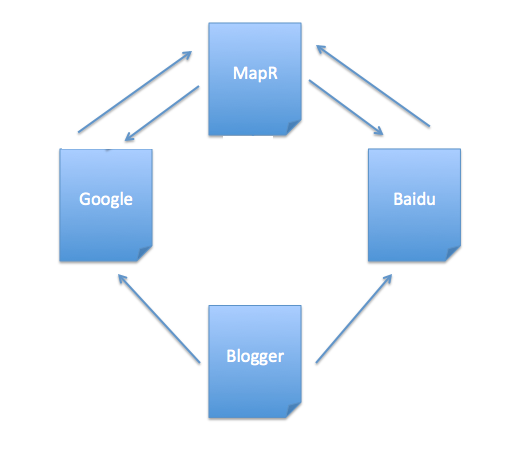
\includegraphics[scale=1.5]{pageRank_4paginas.png}
\end{center}

Las flechas indican los enlaces que hay en cada página.
Se supone que inicialmente hay 1/4 del total de personas en cada una de las 4 páginas.

Hallar la matriz de Markov y determinar, si existe, $\pib^{(\infty)}$ en cada caso.
\begin{enumerate}
\item Considerando que cada minuto, los navegantes clickean alguno de los links al azar disponibles en la página que se encuentran.
\item Considerando que cada minuto, la mitad de los  navegantes que están en una página se quedan en esa página y la otra mitad clickean alguno de los links al azar disponibles en la página que se encuentran.
\end{enumerate}

\end{ejercicio}
